\documentclass[a4paper,english]{report}
\usepackage[utf8]{inputenc}
\usepackage[french]{babel}
%\usepackage[cyr]{aeguill}



\usepackage[a4paper]{geometry}
\geometry{verbose,tmargin=3cm,bmargin=3cm,lmargin=3cm,rmargin=3cm}


%\usepackage{textcomp}

\usepackage{graphicx,epstopdf}% convert eps to pdf
\usepackage[section]{placeins}% allow graph in section


\usepackage{xcolor} 
%\usepackage{pdfpages}% add pdf pages
\usepackage{multicol}% create simpli column
\usepackage{float}
\pagenumbering{arabic} % numerotation des pages
\pagestyle{empty} %No headings for the first pages.

%\usepackage{cite}% bibtex
\usepackage{todonotes}% insert todo

\usepackage{mathtools}
\DeclarePairedDelimiter\abs{\lvert}{\rvert}% abs function

\usepackage{hyperref}% hyperlien
\usepackage{textcomp} % euro symbole

%\usepackage{glossaries}
%\makeglossaries
%%%%% numbering
\usepackage{etoolbox}
\tracingpatches
\makeatletter
\newcommand{\makeCondensedChap}{%
	\patchcmd{\@makeschapterhead}{\vspace*{50\p@}}{}{}{}%
	\patchcmd{\@makeschapterhead}{\vskip 40\p@}{}{}{}%
}
%%%%%reduce spacing
\def\@makechapterhead#1{%
	%%%%\vspace*{50\p@}% %%% removed!
	{\parindent \z@ \raggedright \normalfont
		\ifnum \c@secnumdepth >\m@ne
		\huge\bfseries \@chapapp\space \thechapter
		\par\nobreak
		\vskip 20\p@
		\fi
		\interlinepenalty\@M
		\Huge \bfseries #1\par\nobreak
		\vskip 40\p@
	}}
	\def\@makeschapterhead#1{%
		%%%%%\vspace*{50\p@}% %%% removed!
		{\parindent \z@ \raggedright
			\normalfont
			\interlinepenalty\@M
			\Huge \bfseries  #1\par\nobreak
			\vskip 40\p@
		}}
		
		\makeatletter
		\let\latexps@plain\ps@plain
		\newcommand{\frontmatter}{\let\ps@plain\ps@empty\pagestyle{empty}}
		\newcommand{\mainmatter}{%
			\let\ps@plain\latexps@plain\pagestyle{plain}%
			\clearpage
			\pagenumbering{arabic}}
		\makeatother
		
		%----------------------------------------------------------------------------------------
		\usepackage{titlesec} % Allows customization of titles
		\renewcommand\thesection{\Roman{section}} % Roman numerals for the sections

		\titleformat{\section}[block]{\large\scshape\centering}{\thesection.}{1em}{} % Change the look of the section titles
		\titleformat{\subsection}[block]{\large}{\thesubsection.}{1em}{} % Change the look of the section titles
		
		\usepackage{fancyhdr} % Headers and footers
		\pagestyle{fancy} % All pages have headers and footers
		

	
		
		\title{				\fbox{\parbox{0.8\textwidth }{\centering Réalisation d'une enceinte\\ 2}}\\ } % Article title
		\author{%
			\textsc{Samuel Dupont}\\ %\thanks{A thank you or further information} \\[1ex] % Your name
			%\normalsize Université du Maine \\ % Your institution
			\normalsize \href{mailto:Samuel.dupont.etu@univ-lemans.fr}{Samuel.dupont.etu@univ-lemans.fr } 
		}
		
		\date{December 28, 2016 \\ Last update: \today}

		
		\begin{document}
			\maketitle
			\frontmatter % begin page without numerotation

				\begin{abstract}
					\noindent 
					
				Ce pdf a pour but de rapporter les différentes étapes de la conception d'une enceinte, en partant du choix des haut-parleurs et en passant par les différentes simulations, le choix des matériaux, leur usinage, l'assemblage des boites, la mise en place de  la partie électronique et les finitions.\\ \\
				Le but est de créer une enceinte bluetooth  mono composé de deux haut-parleurs large bande, en s'inspirant du design proposé par la chaine youtube "Les frères Poulains" \href{https://www.youtube.com/watch?v=ollr-PpCMAw}{"Les frères Poulains}. \\

				\end{abstract}
			

			
			\chapter{Introduction}
			Le but est de créer une enceinte bluetooth  mono composé de deux haut-parleurs large-bandes, en s'inspirant du design proposé par la chaine youtube \href{https://www.youtube.com/watch?v=ollr-PpCMAw}{"Les frères Poulains}. \\
			Au lieu d'utiliser le design complet proposé sur la chaine, qui utilise des haut-parleurs de qualité relativement faible, on propose de refaire les simulations en utilisant les conseils du livre de Dickason "Loudspeaker cookbook" ainsi que le logiciel Akabak et ABEC. Nous allons réaliser une enceinte basse réflex.\\
			L'intérêt de n'utiliser qu'un seul type de haut parleur, c'est que l'on n'a pas besoin de traitement sur le son avant d'envoyer au HP contrairement à une enceinte bi-voie (ou plus) où l'on doit séparer le contenu fréquentiel avant d'envoyer sur chaque voie. On a par contre pas l'avantage d'avoir réponse en fréquence qui couvre tout le spectre audible (20~Hz-20~kHz). On vise une enceinte 90~100Hz-17~kHz.\\
			Une fois l'enceinte créé nous avons pour but d'utiliser un raspberry-pi et un DAC audio pour gérer la réception bluetooth. 		
			
			\chapter{Bilan matériel}
			\section{Outils}
			\begin{itemize}
				\item Scie circulaire;
				\item Défonceuse;
				\item Guide plat (planche plate);
				\item Serre joints;
				\item Presses carrés;
				\item Presses d'angles;
				\item Perceuse;
				\item Rouleau à peinture;
			\end{itemize}
			
			\section{Budget}
			Les haut parleurs ont été acheté sur \href{http://loudspeakerfreaks.com/intro.asp}{Loudspeakerfreaks.com}:
			\begin{itemize}
				\item 2 haut parleurs \texteuro;
				\item 1 Raspberry Pi;
				\item 1 DAC audio;
				\item 
			\end{itemize}
			Pour la partie construction:
			\begin{itemize}
				\item Planche de bois massif 18mm;  
				\item Colle, joint, pied, tampon;
				\item Mousse acoustique;
				\item temps passé 0\texteuro.				
			\end{itemize}
			
			\chapter{Réalisation}
			
			\section{Choix des Haut-parleurs}
			Sur le site, une large proposition de haut-parleurs (HP) est présente, on cherche un HP entre 20 et 40\texteuro unité, large bande, en 8 $\Omega$, ce qui nous laisse environ une quinzaine de HP.  On préfère se diriger vers des HP de taille moyenne  ~10cm de diamètre, les gros HP ayant une mauvaise directivités et ne pouvant reproduire les hautes fréquences (HF), tandis que les petits ne peuvent produire des basses fréquences (BF).\\
			En regardant les réponse en fréquence des HP restant on restreint le choix à 4 HP:
			\begin{itemize}
				\item N90 8;
				\item PA100;
				\item PA130;
				\item RS100.
			\end{itemize}
			
			\section{Simulation}
			\subsection{Simulation basiques: Akabak}
			La première étape après les hauts parleurs de choisit, est de démarrer les simulations. On utilise Akabak comme premier jet à partir du livre de Vance Dickason. On peux ainsi voir la réponse en fréquence avec différents volumes d'enceintes et tailles d'évents pour les différents HP.\\ 
			
				La figure \ref{simubassr} les résultats produit par akabak d'une enceinte bass reflex pour 3 différentes configurations pour les différents HP. Les simulations montrent que la configuration C4 qui a un volume de 8L calculé semble acceptable. L'évent est calculé pour un diamètre de 5cm et une résonance de 70Hz, la longueur correspondante est de 12cm.\\
				Les résultats peuvent sembler mauvais, cependant la partie à actuellement considéré est la zone basse fréquence qui est relativement bien représenté dans le modèle du logiciel. Le milieu de la courbe présente des résonances possibles (version non définitive) de la boite, elles sont néanmoins amorties dans la réalité par la mousse et l'amortissement naturel de la boite. Pour la partie haute fréquence (>1000 Hz), le modèle utilisé par le logiciel n'est plus suffisant, et ne représente pas la réalité.
			\begin{figure}[H]
				\centering
				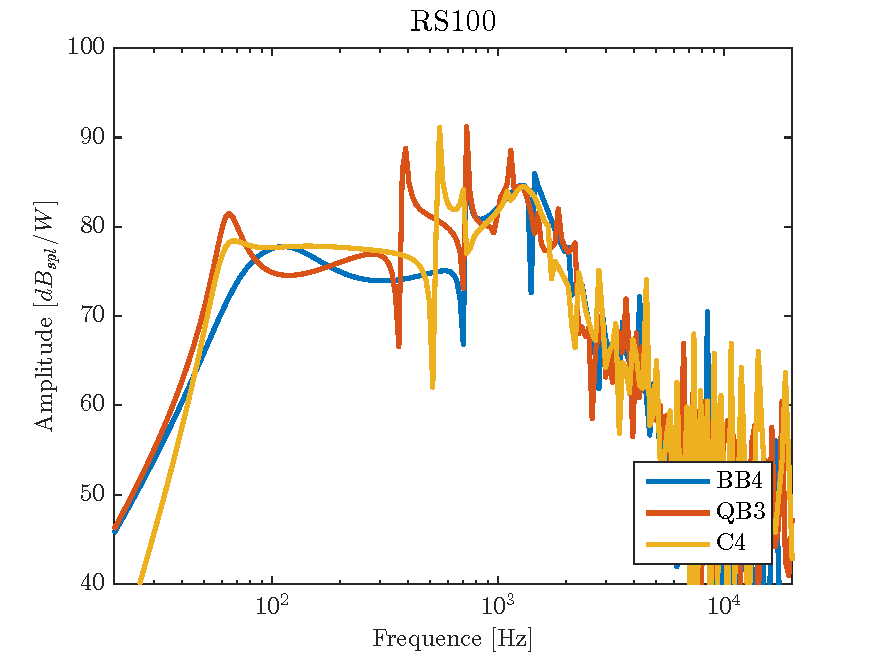
\includegraphics[width=480px]{./Simulation/Akabak/simuAkabak.pdf}
				\label{simubassr}
				\caption{Simulation Akabak Bass reflex}
			\end{figure}


			\section{Simulation avec Abec}
			Dans un second temps, j'utilise Abec3 pour affiner les simulations avec le HP RS100, ce qui permet de calculer la réponse de l'enceinte en prenant en compte les réflexions de la structure et les résonances internes.\\
			Dans un premier temps, il faut établir la géométrie de l'objet en trois dimensions, le visuel correspondant est donnée dan sla Figure 
			\chapter{Conception}
					  
			 	
			
			\section{Planches de bois}

			
			\section{Découpe des ronds}

				\begin{figure}[H]
					\centering
%					\includegraphics[scale=0.25]{./image/DSC_0200b.JPG}
					\label{Planche}
					\caption{Trou des HP}
				\end{figure}			
			

			
			\section{Pré trous de vissage}

			\section{Assemblage de la boite pour tweeter}

		
			    \begin{figure}[h!]
					 	
					 	\begin{minipage}[c]{.45\linewidth}
					 		\begin{center}
%					 			\includegraphics[scale=0.2]{./image/DSC_0198b.JPG}
					 			\label{Boite tweeter}
					 			\caption{Boite tweeter}
					 		\end{center}
					 	\end{minipage}
					 	\hfill
					 	\begin{minipage}[c]{.45\linewidth}
					 		\begin{center}
%					 		\rotatebox{90}{\includegraphics[scale=0.2]{./image/DSC_0202b.JPG}}
					 		\label{Ajout du boite tweeter}
					 		\caption{Ajout du boite tweeter}
					 		\end{center}
					 	\end{minipage}
					 \end{figure} 	
			
			\section{Assemblage de la boite principale}

				\begin{figure}[H]
					\centering
%					\includegraphics[scale=0.3]{./image/DSC_0203b.JPG}
					\label{Boite principlae}
					\caption{Boite principale}
				\end{figure}			
			 
			\section{Ajustement}

			\section{Joint}

			\section{Peinture}

			\section{Remplissage}

			\section{Partie électronique}

		
			\begin{figure}[H]
				\centering
%				\includegraphics[scale=0.3]{./image/filter.JPG}
				\label{Filtre d'une enceinte}
				\caption{Filtre d'une enceinte}
			\end{figure}			
		\chapter{Conclusion}


		
			
			
		\end{document} 